%----------------------------------------------------------------------------------
%----------------------------------SENSIBL-----------------------------------------
%----------------------------------------------------------------------------------
\subsection{Sensitivity analysis}
\subsubsection{Monte-Carlo Sampling and statistical estimations}
\label{subsub:MC}
The Monte Carlo method requires random generation of input variables from their probability distributions. The resulted sampling of a given size $N$ is a $N \times V$ matrix, $V$ being the number of uncertain parameters.  Each row of the matrix $x^i=(x_1,...,x_V)^i$ represents a possible configuration for the coupled hydro-morphodynamic simulation. Corresponding realizations of the output are generated by successive deterministic simulations with each configuration of the inputs. Statistical estimators of the response $Y=(Y_1,...,Y_N) = (M(x^i))_{i \in \{1,...,N\}}$ can therefore be computed from the output as follows :  \\ \\
\textbf{Mean :}
\vspace{-0.7cm}
\begin{equation}
E[Y]=\mu_{Y} = \dfrac{1}{N}\sum_{i=1}^{N} M(x^{i})
\label{eq_moy}
\end{equation}
\\
\textbf{Variance :}
\vspace{-0.9cm}
\begin{equation}
 \quad Var(Y) = \dfrac{1}{N-1}\sum_{i=1}^{N} [M(x^{i})-\mu_{Y}]^{2}
\label{eq_var}
\end{equation}
\\
\textbf{Standard deviation :}
\vspace{-0.7cm}
\begin{equation}
 \qquad \sigma_Y = \sqrt{Var(Y)}
\label{eq_dev}
\end{equation}
These statistical moments are useful for both the uncertainty sensitivity analysis and uncertainty propagation.

The convergence order of the Monte-Carlo sampling method is given by the Central Limit Theorem \cite{bib16} as $\mathcal{O}\left(\dfrac{1}{\sqrt N}\right)$. The estimated statistics are also random quantities and are impacted by estimation uncertainties. Confidence intervals on estimators should therefore be calculated. The non-parametric "bootstrap" method provides information about the statistics uncertainties given few hypothesis \cite{bib1}. Let $x=(x_1,...,x_N)$ denote a sample of $N$ independent and identically distributed realizations according to a probability density function $f(x)$. The statistical moment $\theta=T(F)$ (mean, variance, etc.), is estimated by $\hat{\theta}=T(\hat{F})$, where $\hat{F}$ is the empirical cumulative density function that gives equal probability $\dfrac{1}{N}$ to each observed value $x_i$ defined by :
\begin{equation}
\hat{F}(x) =\dfrac{1}{d} \sum_{i=1}^N 1_{x_i\leq x}
\end{equation}
The idea of the non-parametric bootstrap is to simulate data from the empirical cumulative density function. Given that $\hat{F}$ is build upon equal probability for the observations $(x_1,...,x_N)$, a sample of same size $N$ from $\hat{F}$ would simply be a selection from $(x_1,...,x_N)$ with repeated values. A number of $B$ samples are generated following this strategy, and estimators properties can therefore be deduced as shown in Figure \ref{fig:algo_boots}.
\begin{figure}[!h]
\centering
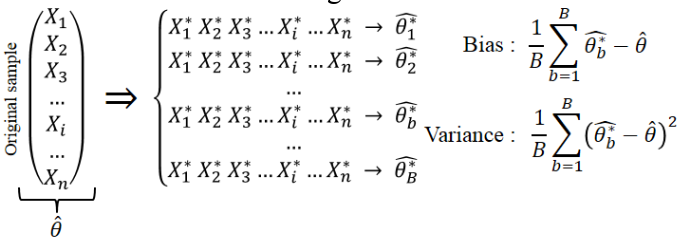
\includegraphics[trim={0 0 0 0.3cm},clip, width=0.5\textwidth]{./Images/bootstrap}
\vspace{-0.5cm}
\caption{Bootstrap algorithm \cite{bib1}}
\label{fig:algo_boots}
\vspace{-0.5cm}
\end{figure}

The confidence interval $I_\theta$ is then estimated as follows :
\begin{equation}
	I_\theta=[0.025-q_{\widehat{\theta}_b},0.975-q_{\widehat{\theta}_b}]
\label{teta_confidence}
\end{equation}
Where $\alpha-q_{X}$ is the $\alpha$-quantile of a variable $X$ defined as :
\begin{equation}
\mathbb{P}(X\leq q_X(\alpha))=\alpha \quad \forall \alpha \in [0,1]
\end{equation}
\subsubsection{Analysis of variance}
\label{subsubsection:ANOVA}
The main goal of a sensitivity analysis is to rank the uncertain parameters according to their influence. In order to do so, a definition of ranking indices is necessary. The indices used here are called Sobol Indices \cite{bib17}.

The definition of Sobol Indices is a result of the ANOVA (Analysis Of VAriance) variance decomposition. In fact, given a set of $V$ \textbf{independent} uncertain parameters $X=(X_1,...,X_V)$, the variance of a response $Y=M(X)$ can be calculated, using the total variance theorem \cite{bib4}, as follows \cite{bib17}: \vspace{-0.2cm}
\begin{equation}
Var[Y] = \sum_{i=1}^{V} \mathcal{V}_i(Y) + \sum_{i<j} \mathcal{V}_{ij}(Y) + ... + \mathcal{V}_{12..V}(Y)
\label{dec_var}
\end{equation}
Where $\mathcal{V}_i(Y)=Var[E(Y|X_i)]$ and $\mathcal{V}_{ij}(Y)=Var[E(Y|X_iX_j)]-\mathcal{V}_i(Y)-\mathcal{V}_j(Y)$, etc. \\ $E(Y|X_i)$ is $Y$'s conditional expectation with the condition that $X_i$ remains constant.

One can therefore calculate first order sensitivity indices that estimate the influence of a variable $X_i$ without its interactions with other variables:
\begin{equation}
S_i = \dfrac{\mathcal{V}_i(Y)}{Var[Y]} = \dfrac{Var(E[Y|X_i])}{Var[Y]}
\label{Sobol_1st}
\end{equation}
And total indices that estimate the global influence of a variable (including interactions):
\begin{equation}
S_{Ti} = S_i + \sum_{j \neq i} S_{ij}  +\sum_{j \neq i, k \neq i, j<k} S_{ijk} + ... = 1 - \dfrac{\mathcal{V}_{-i}(Y)}{Var[Y]}
\label{Sobol_total}
\end{equation}
$\mathcal{V}_{-i}(Y)$ being conditional expectations variances that do not involve $X_{i}$. \\

%----------------------------------------------------------------------------------
\subsubsection{Numerical estimation of indices}
There are two ways to estimate the Sobol indices defined in equations \ref{Sobol_1st} and \ref{Sobol_total} :\\


%-----------------------------------------------------------------------------------------------
\textbf{SALTELLI method \cite{bib16}:}
Step 1:
Two independent samples A and B of size $N$ are generated for the $V$ uncertain variables. For example, sample A can be written as follows:
\begin{equation}
A = \begin{pmatrix}
x_{1}^{A,1} & x_{2}^{A,1} & ... & x_{V}^{A,1} \\
x_{1}^{A,2} & x_{2}^{A,2} & ... & x_{V}^{A,2} \\
 \vdots & \vdots & \ddots & \vdots \\
x_{1}^{A,N} & x_{2}^{A,N} & ... & x_{V}^{A,N} \\
\end{pmatrix}
\end{equation}
A new sample $C$ is created using columns of B except for column $i$ that is replaced with data from A:
\begin{equation}
C = \begin{pmatrix}
x_{1}^{B,1} & ... & x_{i}^{A,1} &... & x_{V}^{B,1} \\
x_{1}^{B,2} & ... & x_{i}^{A,2} &... & x_{V}^{B,2} \\
 \vdots &  & \vdots & & \vdots \\
x_{1}^{B,N} & ... & x_{i}^{A,N} &... & x_{V}^{B,N} \\
\end{pmatrix}
\end{equation}
Simulations using the samples A, B and C result with :
\begin{equation}
\left\{
	\begin{array}{rcr}
	y_k^A = M((x_{1}^{A,k}, ..., x_{V}^{A,k})) \qquad k=\{1,N\} \\
	y_k^B = M((x_{1}^{B,k}, ..., x_{V}^{B,k})) \qquad k=\{1,N\} \\
	y_k^C = M((x_{1}^{C,k}, ..., x_{V}^{C,k})) \qquad k=\{1,N\}
	\end{array}
\right.
\end{equation}
Which can be used to estimate Sobol indices as follows:
\begin{equation}
S_i = \dfrac{\frac{1}{N}\sum_{k=1}^N y_k^A y_k^C - (\mu_{Y^A})^2}{\sigma_{Y^A}^2}
\vspace{-0.2cm}
\end{equation}
\begin{equation}
S_{Ti} = 1-\dfrac{\frac{1}{N}\sum_{k=1}^N y_k^B y_k^C - (\mu_{Y^B})^2}{\sigma_{Y^B}^2}
\end{equation}
Overall, for a given sample size $N$, $(V + 2)\times N$ simulations are necessary to estimate the first order and total Sobol indices for each variable $X_i$. \\

%----------------------------------------------------------------------------------
\textcolor{red}{\textbf{Bootstrap on Saltelli estimation of Sobol indices :} } \\

%--------------------------------------------------------------------------------------------
\textbf{Polynomial chaos method (PCE):} The models response can be approached by an analytical function :
\begin{align*}
M(X) = M_{0} + \sum_{i=1}^V M_i(X_i) + \sum_{1 \leq i < j \leq V} M_{i,j}(X_i,X_j) \\ 
+  \quad ... \quad + M_{1,...,V}(X_1,...,X_V) \addtocounter{equation}{1}\tag{\theequation}
\end{align*} 
$M_i(X_i)$ represents the variable $X_i$'s contribution to the result of the simulation. The variance can therefore be calculated as follows \cite{bib4}:
\begin{align*}
Var[Y] = \sum_{u \subseteq \{1,...,V\}} [ Var[M_u(X_u)] + \\
\sum_{v \subseteq \{1,...,V\}, v \cap u = \emptyset} Cov\left[M_v(X_v), M_u(X_u)\right]] \addtocounter{equation}{1}\tag{\theequation}
\end{align*}
In this particular case of independent variables, the covariance term $Cov\left[M_v(X_v), M_u(X_u)\right]$ vanishes, and the decomposition becomes then equal to ANOVA. Sobol indices can therefore be estimated as:
%\begin{table}[!h]
%\centering
%\begin{tabular}{ccc}
%$S_i = \dfrac{Var\left[M_i(X_i)\right]}{Var[Y]}$ &
%and &
%$S_{Ti} = \dfrac{\sum_{u \subseteq\{1,...,V\}, i \in u} Var\left[M_u(X_u)\right]}{Var[Y]}$
%\end{tabular}
%\vspace{-0.5cm}
%\end{table}
\begin{equation}
S_i = \dfrac{Var\left[M_i(X_i)\right]}{Var[Y]}
\end{equation}
\begin{equation}
S_{Ti} = \dfrac{\sum_{u \subseteq\{1,...,V\}, i \in u} Var\left[M_u(X_u)\right]}{Var[Y]}
\end{equation}
The contributions $M_i(X_i)$ can be calculated by estimating the models response using a polynomial chaos expansion, which can, in a simplified way, be written as:
\begin{equation}
M(X) = \sum_{|\alpha | \leq P} a_\alpha \Psi_\alpha (X)
\end{equation}
Where  $\{ \Psi_\alpha,\alpha \in \mathbb{N}^V \}$ is a multivariate polynomial basis and $a_\alpha$ adequate coefficients for the estimation of the model's response, that can be determined using projection methods \cite{bib4}.

The $X_i$-univariate polynomials shares are the exact contribution of $X_i$ to the polynomial expansion, and are therefore an estimation of $M_i(X_i)$. \\

%----------------------------------------------------------------------------------
\textcolor{red}{\textbf{Bootstrap on Polynomial chaos calculation of Sobol indices :} } \\

%----------------------------------------------------------------------------------


